\begin{center}
  \Large
  \textbf{BIOGRAFI PENULIS}
\end{center}

\addcontentsline{toc}{chapter}{BIOGRAFI PENULIS}

\vspace{2ex}

\begin{wrapfigure}{L}{0.3\textwidth}
  \centering
  \vspace{-3ex}
  % Ubah file gambar berikut dengan file foto dari mahasiswa
  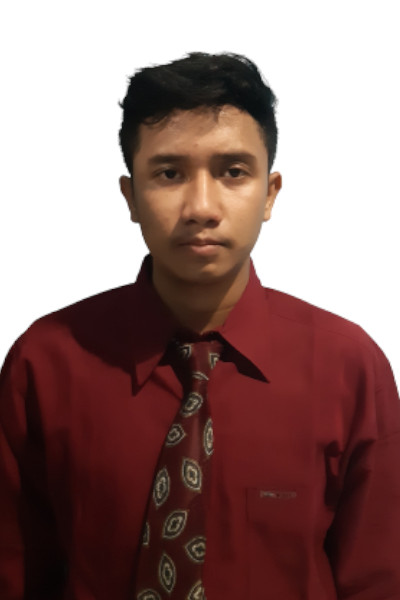
\includegraphics[width=0.3\textwidth]{gambar/helmika_2020pas.jpg}
  \vspace{-4ex}
\end{wrapfigure}

% Ubah kalimat berikut dengan biografi dari mahasiswa
\par Helmika Mahendra Priyanto yang juga biasa dipanggil Helmika lahir di Kota Mataram,
Nusa Tenggara Barat pada tanggal 27 Desember 1999. Pindah ke Kota Semarang Jawa Tengah
pada tahun 2007. Lulus dari SMP Negeri 3 Semarang dan dilanjutkan ke SMA Negeri 3 Semarang.
Pada masa SMA ini lah penulis mulai menyelami dunia programming terutama di bidang \emph{Game Development}.
Setelah lulus dari SMA, penulis menlanjutkan ke perguruan tinggi di Departemen Teknik Komputer di
Institut Teknologi Sepuluh Nopember Surabaya.  Pada masa kuliah, penulis berpartisipasi di beberapa
orgnasisasi seperti Himpunan Mahasiswa Teknik Elektro dan dilanjutkan ke Himpunan Mahasiswa Teknik Komputer.
Penulis juga ikut serta dalam beberapa perlombaan yang berhubungan dengan pengembangan game seperti MAGE ITS, Compfest,
HOLOGY UB, dan GEMASTIK. Selain itu, penulis juga mengikuti program Google Bangkit 2020 dari Kampus Merdeka
dan mulai mempelajari dunia \emph{Cloud Computing}.
